\documentclass[13pt,oneside]{book}
\usepackage[utf8]{inputenc}
\usepackage{url}
\usepackage{graphicx}

\usepackage{geometry}
\geometry{a4paper, left=20mm, right=20mm, top=20mm, bottom=20mm}
\usepackage[margin=1.2in]{geometry}
\usepackage[toc,page]{appendix}
\usepackage{graphicx}
\usepackage{natbib}
\usepackage{lipsum}
\usepackage{caption}

\begin{document}

\captionsetup[figure]{margin=1.5cm,font=small,labelfont={bf},name={Figure},labelsep=colon,textfont={it}}
\captionsetup[table]{margin=1.5cm,font=small,labelfont={bf},name={Table},labelsep=colon,textfont={it}}
\setlipsumdefault{1}

\begin{titlepage}
\begin{center}
{\LARGE College Of Engineering Trivandrum}\\[3cm]
\linespread{1.2}\huge {\bfseries Application Software Development Lab}\\[3cm]
\linespread{1}

\includegraphics[width=5cm]{img/emblem.jpeg}\\[3cm]
{\Large Gokul K\\ S5  CSE \\ Roll No:21\\ TVE18CS021 }\\[1cm]


\textit{ }\\[2cm]
Department of Computer Science\\[0.2cm]
\today
\end{center}

\end{titlepage}

\newpage

\begin{frame}{}
    \centering
    \hspace*{-0.5cm}
    $\vcenter{\hbox{
\includegraphics[width=1.5cm]{img/emblem.jpeg}}}$
    $\vcenter{\resizebox{0.95\textwidth}{!}{
        \begin{tabular}{c}
             CS333 - Application Software Development Lab $\cdot$ 2020 $\cdot$   \\
             \hline 
        \end{tabular}
    }}$
\end{frame}
\section*{Cycle 2}
\section*{Expt 2}
\begin{center}
    \Large{CURSOR}
\end{center}

\section*{Aim}
\large To study the use and implementation of cursors in PL/SQL.
\section*{QUESTIONS:}
\begin{itemize}
    \item
    Create table student (id, name, m1, m2, m3, grade).Insert 5 tuples into it. Find the total,
     calculate grade and update the grade in the table.
     
    Syntax:
    \begin{verbatim}
    CREATE TABLE student (
            id INT,
        name VARCHAR,
            m1 INT,
            m2 INT,
            m3 INT,
            grade CHAR
    );
    INSERT INTO student
    (id, name, m1, m2, m3) VALUES
            (10, 'Name1', 58, 61, 29),
            (30, 'Name2', 60, 60, 60),
            (12, 'Name3', 50, 67, 75),
            (13, 'Name4', 59, 69, 99),
            (21, 'Name5', 10, 99, 10);
    SELECT * FROM student;
    CREATE OR REPLACE FUNCTION calculate_grade() RETURNS VOID AS $$
    DECLARE
            total INT;
            grde CHAR;
            record_student RECORD;
            cursor_student CURSOR
            FOR SELECT * FROM student;
    BEGIN
            OPEN cursor_student;
            LOOP
                    FETCH cursor_student INTO record_student;
                    EXIT WHEN NOT FOUND;
                    total = record_student.m1 + 
                    record_student.m2 + record_student.m3;
                    IF total > 240 THEN grde = 'A';
                    ELSIF total > 180 THEN grde = 'B';
                    ELSIF total > 120 THEN grde = 'C';
                    ELSIF total > 60 THEN grde = 'D';
                    ELSE grde = 'F';
                    END IF;
                    UPDATE student SET grade=grde WHERE id=record_student.id;
            END LOOP;
            CLOSE cursor_student;
    END;
    $$ LANGUAGE plpgsql;
    SELECT calculate_grade();
    SELECT * FROM student;
    
    \end{verbatim}
    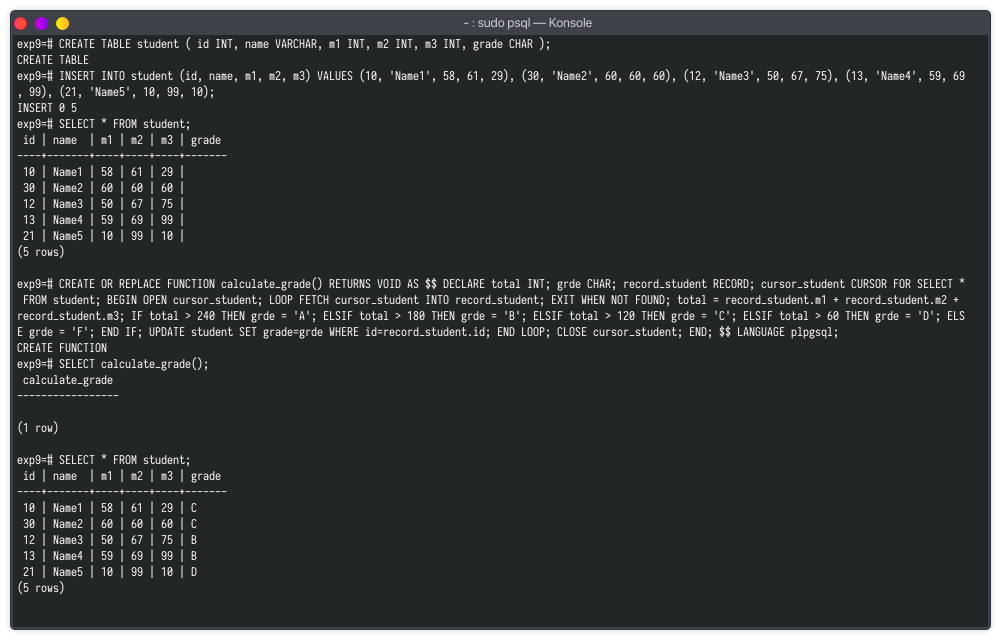
\includegraphics[width=\textwidth]{img/p9/ss1.png}
    
    
    \item
    Create bank details(accno, name, balance,adate).Calculate the interest of the amount and
     insert into a new table with fields(accno, interest). Interest= 0.08*balance.
     
    Syntax:
    \begin{verbatim}
    CREATE TABLE bank_details (
            accno INT,
            name VARCHAR(10),
            balance INT,
            adate DATE
    );
    CREATE TABLE bank_interest (
            accno INT,
            interest REAL
    );
    INSERT INTO bank_details 
    VALUES
            (1001, 'Name1', 20000, '10-DEC-2019'),
            (1012, 'Name2', 25000, '17-APR-2019');
    CREATE OR REPLACE FUNCTION calculate_interest()
    RETURNS VOID AS $$
    DECLARE
            interest INT;
            account RECORD;
            account_cursor CURSOR
            FOR SELECT * FROM bank_details;
    BEGIN
            OPEN account_cursor;
            LOOP
                    FETCH account_cursor INTO account;
                    EXIT WHEN NOT FOUND;
                    interest = 0.8*account.balance;
                    INSERT INTO bank_interest VALUES (account.accno, interest);
            END LOOP;
            CLOSE account_cursor;
    END;
    $$ LANGUAGE plpgsql;
    SELECT calculate_interest();
    SELECT * FROM bank_interest;
    
    \end{verbatim}
    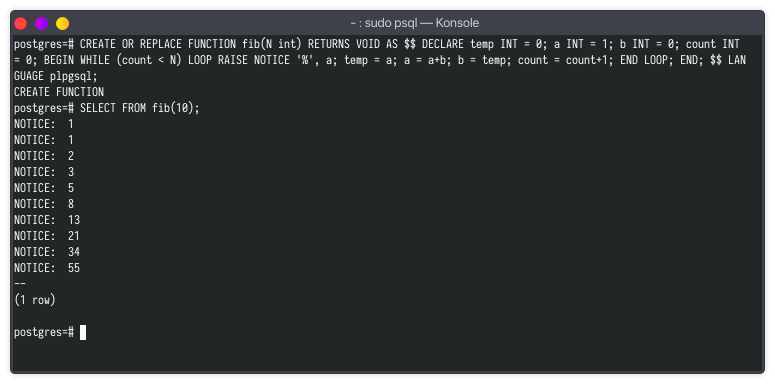
\includegraphics[width=\textwidth]{img/p9/ss2.png}
    
    
    \item
    Create table people\_list(id, name, dt\_joining, place).
    If persons experience
     is above 10 years, put the tuple in table exp\_list(id, name, experience).
     Create table employee list(id,name,monthly salary).\\
     i) If: annual salary less than 60000, increment monthly salary by 25\% \\
     ii) between 60000 and 200000, increment by 20\% \\
     iii) between 200000 and 500000, increment by 15\% \\
     iv) annual salary greater than 500000, increment monthly salary by 10\%.
    
    Syntax:
    \begin{verbatim}
    CREATE TABLE people_list (
            id INT,
            name VARCHAR(10),
            dt_joining DATE,
            place VARCHAR(5)
    );
    CREATE TABLE exp_list(
            id INT,
            name VARCHAR,
            experience INT
    );
    INSERT INTO people_list
    VALUES
            (101, 'Name1', '10-APR-2020', 'City1'),
            (101, 'Name2', '10-APR-2010', 'City2'),
            (101, 'Name3', '10-APR-2000', 'City3');
    SELECT * FROM people_list;
    CREATE OR REPLACE FUNCTION calculate_exp()
    RETURNS VOID AS $$
    DECLARE
            exp INT;
            person RECORD;
            today DATE;
            person_cursor CURSOR FOR SELECT * FROM people_list;
    BEGIN
            OPEN person_cursor;
            SELECT current_date INTO today;
            LOOP
                    FETCH person_cursor INTO person;
                    EXIT WHEN NOT FOUND;
                    SELECT DATE_PART('year', today::date) 
                    - DATE_PART('year', person.dt_joining::date)
                    INTO exp;
                    IF exp > 10 THEN
                            INSERT INTO exp_list 
                            VALUES (person.id, person.name, exp);
                    END IF;
            END LOOP;
            CLOSE person_cursor;
    END;
    $$ LANGUAGE plpgsql;
    SELECT calculate_exp();
    SELECT * FROM exp_list;
    \end{verbatim}
    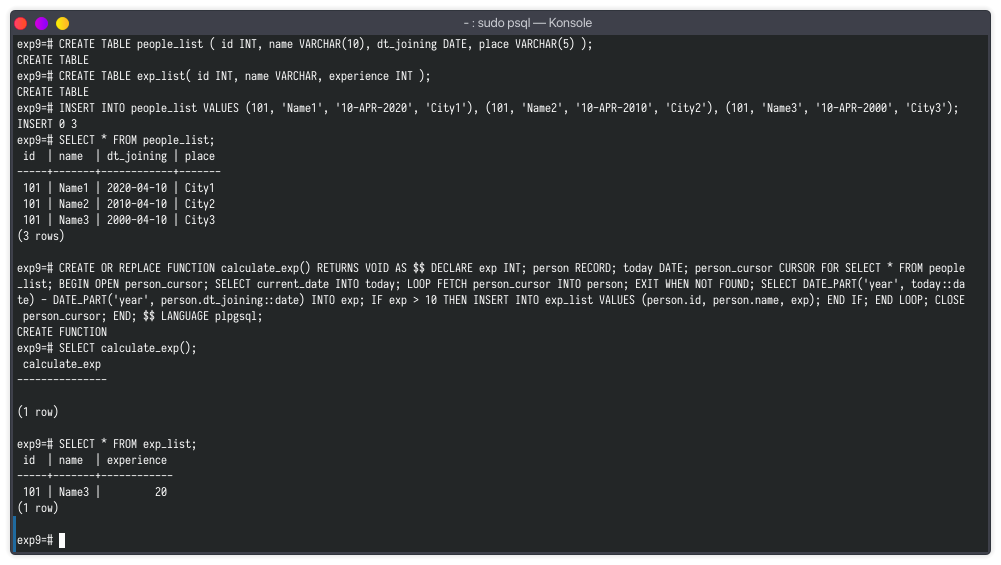
\includegraphics[width=\textwidth]{img/p9/ss3.png}
\end{itemize}
\section*{Result}
Implemented the PL/SQL CURSOR programs in Postgres SQL in Linux and following Output were obtained.
\end{document}